\documentclass[a4paper,8pt,openany]{book}
\usepackage[utf8]{inputenc}
\usepackage[french]{babel}
\usepackage[T1]{fontenc}
\usepackage{graphicx}
\usepackage{titlesec}
\usepackage{comment}
\usepackage{amsmath}
\usepackage{amsfonts}

\titleformat{\chapter}[block]
  {\normalfont\Huge\bfseries}% font of number
  {\chaptertitlename\ \thechapter~:}% format of number
  {20pt}% space between number and title
  {\Huge}% font of title

\titlespacing*{\chapter}
  {0pt}%  indent
  {0pt}% space before
  {20pt}% space after
\titlespacing*{\section}
  {0pt}%  indent
  {3.5ex plus 1ex minus .2ex}% space before
  {2.3ex plus .2ex}% space after

\author{Mendy Fatnassi}
\title{Les fonctions en mathematique}

%%%%%%%%%%%%%%%%%%%%%%%%%%%%%%%%%%%%%%	Page	%%%%%%%%%%%%%%%%%%%%%%%%%%%%%%%%%%%%%%%%
\begin{document}
\maketitle
\tableofcontents

%%%%%%%%%%%%%%%%%%%%%%%%%%%%%%%%%%%%%%%%%%%%%%%%%%%%%
\chapter{Les Fonctions}

\section{Notion de fonction}
Une fonction f(x) possede une image et un antecedant .L'image seras le resultat de x a travers f(x) et l'antecedant seras pour quelle x on obtient un resultat y , f(?)=y.\\
Par exemple f(5):-> 25 , l'image de f(5) est 25 et l'antecedant de 25 est f(5).\\
\\
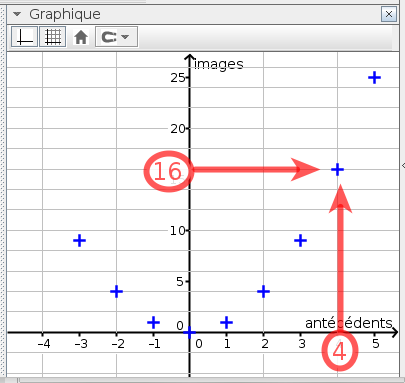
\includegraphics[width=0.60\textwidth, center]{img/img_ant_graph.png}\\
\\
On peux aussi resoudre une equation graphiquement , par exemple :\\
$f(x) = 5x-x^2$ , on cherche f(2) donc $f(x)=2 => 5x-x^2=2$ :\\
\\
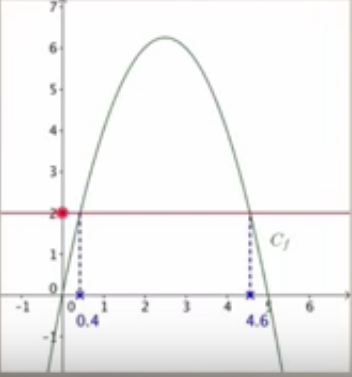
\includegraphics[width=0.60\textwidth, center]{img/resol_equ_graph.png}\\


\section{Fonction affine & polynome du 2nd degré}

\subsection{Fonction affine}
Une fonction f définie sur R est une fonction affine si elle peut s’écrire sous la forme $f(x) = ax + b$ avec a et b réels.\\
avec a: le coef. directeur et b: l'ordonnée a l'origine.\\
\\
Une fonction affine est graphiquement representer par une droite qui n'est pas parrallele a l'axe des ordonné.  Il y a deux cas particuliers importants de fonctions affines : $f(x) = ax + b$\\
\\
Si b = 0, c’est-à-dire, f(x) = ax ; alors f est appelée fonction linéaire.\\
Si a = 0, c’est-à-dire, f(x) = b ; alors f est une fonction constante.\\



\subsection{Fonction du 2nd degré}
Si la fonction possede 3 coef. a,b et c on parleras d'equation du second degré .Ces fonctions sont representer graphiquement par une parabole .\\
Pour calculer un polynome du 2nd degré on applique la formule : $\Delta$ $=b^2-4ac$ : \\
\\
- Si $\Delta$ > 0 alors 2 solution : $x1=\frac{-b-\rac{\Delta}}{2a}$ et $x2=\frac{-b+\rac{\Delta}}{2a}}$\\
\\
- Si $\Delta$ = 0 alors 1 solution : $x1=\frac{-b}{2a}$\\
\\
- Si $\Delta$ < 0 alors il n'y a pas de solution réel.\\
 

\section{limite de fonction}
Si on veux trouver la limite pour un x donnée , $\lim\limits_{x \rightarrow 4}2x-7$ et bien on remplace le x de la fonction par 4 (ce quoi il tend) :\\
\\
$\lim\limits_{x \rightarrow 4}2x-7 = 2\times4-7=1$ on dit que la limite de la fonction 2x-7 quand x tend vers 4 est 1 .\\
\\
Pour les limite en $+/- \infty$ on ne remplace pas x par $\infty$ car cela n'est pas possible .On vas donc regarder :\\
$\lim\limits_{x \rightarrow 0+} f(x) = +\infty$ et $\lim\limits_{x \rightarrow 0-} f(x) = -\infty$ \\
\\
\underline{Forme Indetermin\'e} : \\
\\
Parfois on fait face a des formes indeterminé que l'on note F.I. On est dans ce cas quand on a par exemple une somme de fonctions, l’une tendant vers $+\infty$ , l’autre vers $-\infty$.\\
Il y a 4 formes indeterminé en tout : \\
\\
$+\infty-\infty$ , $0 \times \infty$ , $\frac{\infty}{\infty}$ et $\frac{0}{0}$\\
\\
Quand on a des polynômes, on peut tomber sur des F.I.
Dans ce cas on utilise le \textbf{TH du plus haut degrés} (seulement si x tend vers $+/-\infty$).\\
\\
\underline{Exemple} : \\
\\
- $\lim\limits_{x \rightarrow +\infty}x^2 -x = +\infty -\infty = F.I $\\
- $\lim\limits_{x \rightarrow +\infty}x^2 -x= \lim\limits_{x \rightarrow +\infty}x^2$\\
- $\lim\limits_{x \rightarrow +\infty}\frac{x^2-x}{9x^5-6x^2+7}= 
\lim\limits_{x \rightarrow +\infty}\frac{x^2}{9x^5}=
\lim\limits_{x \rightarrow +\infty}\frac{1}{9x^3}=0$\\
\\
Grace aux limites on pourras completer le tableau de signe d'une fonction en y ajoutant les limites de x en $+/-\infty$ .\\
\\
Pour $x^2-4x+3$ on a :\\
\\
- $\lim\limits_{x \rightarrow +\infty}x^2-4x+3=+\infty$\\
- $\lim\limits_{x \rightarrow -\infty}x^2-4x+3=+\infty$\\
\\
\\
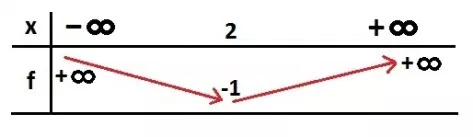
\includegraphics[width=0.60\textwidth, center]{img/limite-tab-variation.png}


\section{dérivée de fonction}
\\
Quand on a une fonction f, on peut calculer une autre fonction que l'on note f' (f prime) et qu'on appelle la dérivée de f .\\
\\
\textbf{Tableau de derivée} :\\
\\
\begin{center}
  \begin{tabular}{|c|c|}
    \hline
    f & f' \\ \hline
    constante & 0 \\ \hline
    x & 1 \\ \hline
    $x^2$ & 2x \\ \hline
    $x^3$ & $3x^2$ \\ \hline
    $x^{n}$ & $n\times x^{n-1}$ \\ \hline
    $\frac{1}{x}$ & $-\frac{1}{x^{2}}$\\ \hline
    $\sqrt{x}$ & $\frac{1}{2\sqrt{x}}$ \\ \hline
    $\sin(x)$ & $\cos(x)$ \\  \hline
    $\cos(x)$ & $-\sin(x)$ \\
    \hline
  \end{tabular}
\end{center}
\\
\underline{Exemple}:\\
\\
$f(x) = 7x^9-8x^3+5$ on vas alors dérivée chacun des termes et les constantes multiplicative sont simplement réecrites dans 
l'équation , ce qui donne :\\
\\
$f'(x)= 7\times9x^8-8\times3x^2+0 \Rightarrow f'(x)=63x^8-24x^2$\\
\\
Par contre si on a des produits ou quotient de fonctions par exemple 2 fonctions u et v (cf.Tableau de derivee complexe).\\
\\
$(u\times v)'=u'v+uv'$\\
\\
$\left(\frac{u}{v}\right)'=\frac{u'v-uv'}{v^2}$\\
\\
\underline{Exemple}:\\
\\
$f(x)=(2x+1)\times(x^2-9)$ pour trouver la dérivée il est conseiller de faire comme suite : \\
\\
$u = 2x +1 et u'=2$  \\
$v = x^2-9 et v'=2x$ \\
\\
Ensuite on remplace les formules dans l'expression de la fonction : \\
\\
$f'(x)=u'v+uv'=(2)\times(x^2-9)+(2x+1)\times(2x)$\\
$f'(x)=2x^2-18+4x^2+2x$\\
$f'(x)=6x^2+2x-18$\\
\\
On appelle cela des fonction composé , elles sont de la forme $f(x)=\sqrt{8x^2-5x+4}$ ou $f(x)=\frac{1}{8x^6+4x^7-6x}$ en generale ces fonction sont noté u , $\sqrt{u}$ ou $\frac{1}{u}$ .\\
\\
Pour derivée ce genre de fonction on derivee le u comme si il s'agissait d'un réel x et on multiplie par u'.\\
\\
\textbf{Tableau de derivee complexe} :\\
\\
\begin{center}
  \begin{tabular}{|c|c|}
    \hline
    f & f' \\ \hline
    $u^2$ & $2u\times u'$ \\ \hline
    $u^3$ & $3u^2\times u'$ \\ \hline
    $u^n$ & $n\times u^{n-1}\times u'$\\ \hline
    $\frac{1}{u}$ & $-\frac{1}{u^2} \times u'$ \\ \hline
    $\sqrt{u}$ & $\frac{1}{2\sqrt{u}}\times u'$ \\ \hline
    $\sin(x)$ & $\cos(x)\times u'$ \\  \hline
    $\cos(x)$ & $-\sin(x)\times u'$ \\
    \hline
  \end{tabular}
\end{center}\\
\\
\underline{Interet}:\\
f' sert a trouver les signes/variations de f .\\
- si f'>=0, alors f est croissante \\
- si f'<=0, alors f est décroissante \\

\section{signes \& variation}
On cherche le tableau de signes de f' pour trouver le tableau de variation de f (\textbf{ne pas melanger f et f'}) , pour cela on calcule d'abord f' .\\
\\
$f(x)=x^2-6x+4$\\
$f'(x)=2x-6$\\
\\
f' est de la forme ax+b , il suffit donc de savoir quand f' s'annule . $2x-6=0 \Rightarrow 2x=6 \Rightarrow x=3$ .\\
\\
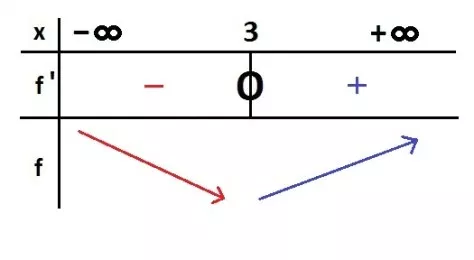
\includegraphics[width=0.5\textwidth , center]{img/tableau-signe-variation.png}


\section{Equation de la tangeante}
Une tangeante c’est une droite, elle est donc de la forme $y = ax + b$ .\\
Ensuite, cette droite \« longe \» la courbe de la fonction sans la traverser.\\
\\
Voici la formule : $y = f'(a)(x-a)+f(a)$\\
\\

\section{Primitive}
Pour faire simple, une primitive c’est \« l’inverse de la dérivée \» \\
$F'(x)=f(x)$\\
F est la primitive de f et f la dérivee de F.Si on dérive f(x) on obtient f'(x) , si on derivee la primitive c-a-d  F'(x) on obtient f(x).\\
\\
\textbf{Tableau de primitive} :\\
\\
\begin{right}
  \begin{tabular}{|c|c|}
    \hline
    f & F \\ \hline
    $0$ & $constante$ \\ \hline
    $x$ & $\frac{x^2}{2}$ \\ \hline
    $x^2$ & $\frac{x^3}{3}$ \\ \hline
    $x^3$ & $\frac{x^4}{4}$ \\ \hline
    $x^n$ & $\frac{x^{n+1}}{n+1}$ \\ \hline
    $x^{-1} $ & $ln(x)$ \\ \hline
    $\frac{1}{x}$ & $\ln{x}$ \\ \hline
    $\frac{1}{x^2}$ & $\frac{-1}{x} $ \\ \hline
    $\frac{1}{2\sqrt{x}}$ & $\sqrt{x}$ \\ \hline
    $e^x$ & $e^x$ \\ \hline
    $\sin(x)$ & $-\cos(x)$ \\  \hline
    $\cos(x)$ & $\sin(x)$ \\
    \hline
  \end{tabular}
\end{right}
\\
\\
\\
\textbf{Tableau de primitive complexe} :\\
\\
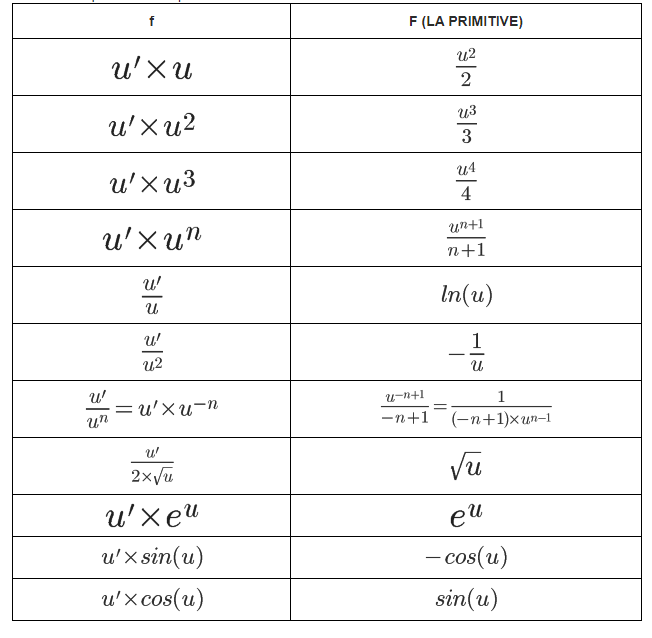
\includegraphics[width=0.65\linewidth ,center]{img/tableau_primitive_complexe.png}
\\


\section{Integrale}\\
Une intégrale c’est l’aire sous la courbe d’une fonction, entre deux points d’abscisses a et b. 
\\
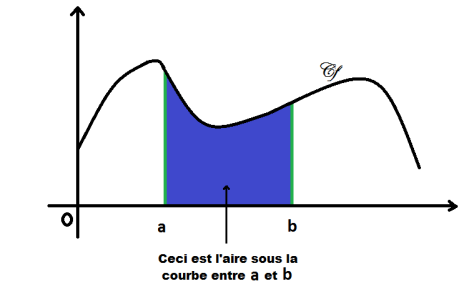
\includegraphics[width=0.65\linewidth ,center]{img/integrale-aire-courbe.png}
\\
\underline{Calcule d'une integrale} : \\
\\
Soient [a, b] un intervalle de R , une fonction continue sur [a, b] et F une primitive de f , on a :\\
\\
$\int_a^b f(x) dx=[F(x)]^b_a=F(b)-F(a)$\\
\\
\underline{Exemple} : \\
\\
Si on veux integrer la fonction $f(x) = \frac{3}{x^2}$ sur l'intervale [1;4] il faut trouver une primitive de f(x) , or $\frac{3}{x^2}$ n'a pas de primitive on peux donc modifier un peux l'ecriture de celle ci $f(x)=3 \times \frac{1}{x^2}$\\
\\
Donc $F(x)=3\times -\frac{1}{x} = -\frac{3}{x}$\\
\\
$\int_1^4 \frac{3}{x^2} = [-\frac{3}{x}]^4_1 = -\frac{3}{4} - (-\frac{3}{1}) = -\frac{3}{4} + \frac{12}{4} = \frac{9}{4} $ \\




\end{document}
